% Options for packages loaded elsewhere
\PassOptionsToPackage{unicode}{hyperref}
\PassOptionsToPackage{hyphens}{url}
\PassOptionsToPackage{dvipsnames,svgnames,x11names}{xcolor}
%
\documentclass[
]{article}

\usepackage{amsmath,amssymb}
\usepackage{iftex}
\ifPDFTeX
  \usepackage[T1]{fontenc}
  \usepackage[utf8]{inputenc}
  \usepackage{textcomp} % provide euro and other symbols
\else % if luatex or xetex
  \usepackage{unicode-math}
  \defaultfontfeatures{Scale=MatchLowercase}
  \defaultfontfeatures[\rmfamily]{Ligatures=TeX,Scale=1}
\fi
\usepackage{lmodern}
\ifPDFTeX\else  
    % xetex/luatex font selection
\fi
% Use upquote if available, for straight quotes in verbatim environments
\IfFileExists{upquote.sty}{\usepackage{upquote}}{}
\IfFileExists{microtype.sty}{% use microtype if available
  \usepackage[]{microtype}
  \UseMicrotypeSet[protrusion]{basicmath} % disable protrusion for tt fonts
}{}
\makeatletter
\@ifundefined{KOMAClassName}{% if non-KOMA class
  \IfFileExists{parskip.sty}{%
    \usepackage{parskip}
  }{% else
    \setlength{\parindent}{0pt}
    \setlength{\parskip}{6pt plus 2pt minus 1pt}}
}{% if KOMA class
  \KOMAoptions{parskip=half}}
\makeatother
\usepackage{xcolor}
\usepackage[margin=0.3in]{geometry}
\setlength{\emergencystretch}{3em} % prevent overfull lines
\setcounter{secnumdepth}{5}
% Make \paragraph and \subparagraph free-standing
\makeatletter
\ifx\paragraph\undefined\else
  \let\oldparagraph\paragraph
  \renewcommand{\paragraph}{
    \@ifstar
      \xxxParagraphStar
      \xxxParagraphNoStar
  }
  \newcommand{\xxxParagraphStar}[1]{\oldparagraph*{#1}\mbox{}}
  \newcommand{\xxxParagraphNoStar}[1]{\oldparagraph{#1}\mbox{}}
\fi
\ifx\subparagraph\undefined\else
  \let\oldsubparagraph\subparagraph
  \renewcommand{\subparagraph}{
    \@ifstar
      \xxxSubParagraphStar
      \xxxSubParagraphNoStar
  }
  \newcommand{\xxxSubParagraphStar}[1]{\oldsubparagraph*{#1}\mbox{}}
  \newcommand{\xxxSubParagraphNoStar}[1]{\oldsubparagraph{#1}\mbox{}}
\fi
\makeatother


\providecommand{\tightlist}{%
  \setlength{\itemsep}{0pt}\setlength{\parskip}{0pt}}\usepackage{longtable,booktabs,array}
\usepackage{calc} % for calculating minipage widths
% Correct order of tables after \paragraph or \subparagraph
\usepackage{etoolbox}
\makeatletter
\patchcmd\longtable{\par}{\if@noskipsec\mbox{}\fi\par}{}{}
\makeatother
% Allow footnotes in longtable head/foot
\IfFileExists{footnotehyper.sty}{\usepackage{footnotehyper}}{\usepackage{footnote}}
\makesavenoteenv{longtable}
\usepackage{graphicx}
\makeatletter
\def\maxwidth{\ifdim\Gin@nat@width>\linewidth\linewidth\else\Gin@nat@width\fi}
\def\maxheight{\ifdim\Gin@nat@height>\textheight\textheight\else\Gin@nat@height\fi}
\makeatother
% Scale images if necessary, so that they will not overflow the page
% margins by default, and it is still possible to overwrite the defaults
% using explicit options in \includegraphics[width, height, ...]{}
\setkeys{Gin}{width=\maxwidth,height=\maxheight,keepaspectratio}
% Set default figure placement to htbp
\makeatletter
\def\fps@figure{htbp}
\makeatother

\usepackage{fvextra}
\DefineVerbatimEnvironment{Highlighting}{Verbatim}{breaklines,commandchars=\\\{\}}
\makeatletter
\@ifpackageloaded{caption}{}{\usepackage{caption}}
\AtBeginDocument{%
\ifdefined\contentsname
  \renewcommand*\contentsname{Table of contents}
\else
  \newcommand\contentsname{Table of contents}
\fi
\ifdefined\listfigurename
  \renewcommand*\listfigurename{List of Figures}
\else
  \newcommand\listfigurename{List of Figures}
\fi
\ifdefined\listtablename
  \renewcommand*\listtablename{List of Tables}
\else
  \newcommand\listtablename{List of Tables}
\fi
\ifdefined\figurename
  \renewcommand*\figurename{Figure}
\else
  \newcommand\figurename{Figure}
\fi
\ifdefined\tablename
  \renewcommand*\tablename{Table}
\else
  \newcommand\tablename{Table}
\fi
}
\@ifpackageloaded{float}{}{\usepackage{float}}
\floatstyle{ruled}
\@ifundefined{c@chapter}{\newfloat{codelisting}{h}{lop}}{\newfloat{codelisting}{h}{lop}[chapter]}
\floatname{codelisting}{Listing}
\newcommand*\listoflistings{\listof{codelisting}{List of Listings}}
\makeatother
\makeatletter
\makeatother
\makeatletter
\@ifpackageloaded{caption}{}{\usepackage{caption}}
\@ifpackageloaded{subcaption}{}{\usepackage{subcaption}}
\makeatother

\ifLuaTeX
  \usepackage{selnolig}  % disable illegal ligatures
\fi
\usepackage{bookmark}

\IfFileExists{xurl.sty}{\usepackage{xurl}}{} % add URL line breaks if available
\urlstyle{same} % disable monospaced font for URLs
\hypersetup{
  pdftitle={PPHA 30538 1- Final Project Writeup},
  pdfauthor={Xinyi Zhou, and Wuzhen Han},
  colorlinks=true,
  linkcolor={blue},
  filecolor={Maroon},
  citecolor={Blue},
  urlcolor={Blue},
  pdfcreator={LaTeX via pandoc}}


\title{PPHA 30538 1- Final Project Writeup}
\author{Xinyi Zhou, and Wuzhen Han}
\date{2024-12-05}

\begin{document}
\maketitle

\RecustomVerbatimEnvironment{verbatim}{Verbatim}{
  showspaces = false,
  showtabs = false,
  breaksymbolleft={},
  breaklines
}


Group Members:

Xinyi Zhou (Github:XinyiZhou66) , Responsible part: line chart, and
shiny app part 2 (Trends in Real GDP and Unemployment Rate\ldots{} )

Wuzhen Han (Github:hanwuzhen), Responsible part: bar chart, and shiny
app part 1 (Unemployment Rate by State- heatmap)

\section{Research Topic: Evaluating the Effectiveness of the CARES Act
in Accelerating Employment Recovery During the COVID-19
Pandemic}\label{research-topic-evaluating-the-effectiveness-of-the-cares-act-in-accelerating-employment-recovery-during-the-covid-19-pandemic}

The goal of this research is to evaluate the effectiveness of the CARES
Act in accelerating employment recovery during the COVID-19 pandemic.
Specifically, we analyzed trends in Real Gross Domestic Product (GDP)
and unemployment rates to determine if the CARES Act, with its economic
stimulus provisions, helped reduce unemployment more effectively
compared to other measures. Our analysis took place at both the national
and state levels, focusing on disparities across states and changes over
time to assess the Act's impact comprehensively.

To conduct our analysis, we utilized multiple data sources. The GDP data
was collected from the Federal Reserve Economic Data (FRED) database,
which provided an accurate representation of the U.S. economy's growth
over time. For unemployment rates, we used two datasets from the Bureau
of Labor Statistics (BLS). The first dataset provided overall yearly
unemployment rates for the entire United States, which we downloaded
directly from the BLS website. The second dataset contained state-level
unemployment rates. Additionally, information on CARES Act funding was
sourced from Treasury Department documents, and geographic data were
collected from the U.S. Census Bureau, which helped facilitate our
state-level analysis.

We conducted Natural Language Processing (NLP) analysis on the CARES Act
report to gain insights. Sentiment analysis helped assess the emotional
tone, capturing polarity and subjectivity. Named Entity Recognition
identified key entities like organizations and locations, while
tokenization and Part-of-Speech tagging provided a detailed breakdown of
the text. This allowed us to better understand the content and overall
narrative of the document.

Our analysis relies on two key assumptions. First, we assume that
changes in unemployment rates and Real GDP are largely due to the CARES
Act, though other factors may also influence these outcomes. We also
assume uniform state responses to the CARES Act, ignoring differences in
local policies and economic conditions.

The research employed quantitative, descriptive, and interactive
analysis to evaluate the impact of the CARES Act. Quantitative analysis
included static visualizations such as bar charts depicting the
distribution of CARES Act funding and line plots of unemployment rates
and Real GDP trends. California, Texas, and New York received the most
funding, and we compared this funding distribution to unemployment
trends to assess recovery. Interactive visualizations provided deeper
insight into economic changes, aiming to offer both macro and detailed
perspectives on the CARES Act's impact during the pandemic. This
dashboard had two main components:

The first component was a heatmap showing state-level unemployment rates
from 2018 to 2024. Users could select different years to observe how
unemployment varied across the United States, highlighting the three
states with the highest rates each year. The second component of our
dashboard focused on broader trends in economic indicators such as Real
GDP and unemployment rates over the same period. This component allowed
users to explore different time periods, such as before the CARES Act
was implemented (2018 Q1 to 2020 Q1), during the CARES Act
implementation (2020 Q2), and after its implementation. These periods
helped illustrate changes over time, such as the initial surge in
unemployment and GDP drop at the start of the pandemic and the
subsequent recovery. The line charts clearly depicted the impact of the
CARES Act's timing on both employment and GDP recovery.

The analysis led to several notable findings. In 2019, unemployment
rates were relatively low. However, in 2020, unemployment surged,
especially in tourism-heavy states like Nevada, Hawaii, and California,
with Nevada reaching 13.5\%. By 2021, unemployment rates declined, with
California dropping from 10.1\% in 2020 to 7.3\%, partly influenced by
the \$193 million it received from the CARES Act. This suggests that
targeted federal aid may have helped mitigate the effects of
unemployment in hard-hit states. Nationally, a vertical dashed line
marked the CARES Act implementation, helping to visualize its impact.
The trend analysis revealed an economic downturn in early 2020, with a
spike in unemployment and a GDP drop. Following the CARES Act, there was
an almost immediate recovery in GDP and unemployment. The interactive
dashboard helped users distinguish short-term improvements from
longer-term trends, showing continued economic recovery. These findings
suggest that the CARES Act was instrumental in stabilizing the economy
and aiding employment recovery, though other factors also contributed.

In our project, one limitation was that we did not account for
population differences when analyzing the distribution of CARES Act
funding. The bar plot presented the total funding received by each
state, meaning that larger states like California and Texas naturally
appeared to receive more. This approach lacks a per capita perspective,
which would have provided more insight into the fairness and
effectiveness of the fund allocation relative to each state's population
and needs. Additionally, our analysis focused primarily on unemployment
rate and Real GDP, while neglecting other important metrics like
inflation rate or household financial stability, which could have
offered a broader understanding of the CARES Act's impact during the
pandemic.

For future work, incorporating econometric models could better help
isolate the impact of the CARES Act from other influencing factors. This
would improve the robustness of our conclusions. Moreover, breaking down
the ``Unemployment Rate by State'' into monthly data for 2021 could
provide insights into how different cities were impacted over time,
capturing the dynamic response in key metropolitan areas. This approach
would allow us to identify whether some cities recovered faster than
others and understand the differential effects within states, offering a
more granular perspective on how effectively the CARES Act supported
various local economies. It would also be valuable to explore other
aspects, such as household financial stability or small business
recovery, to gain a broader understanding of the CARES Act's influence
during the pandemic.

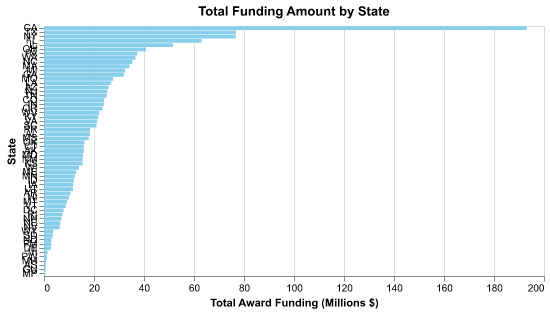
\includegraphics[width=5.72917in,height=3.26042in]{write_up_files/figure-pdf/cell-5-output-1.png}

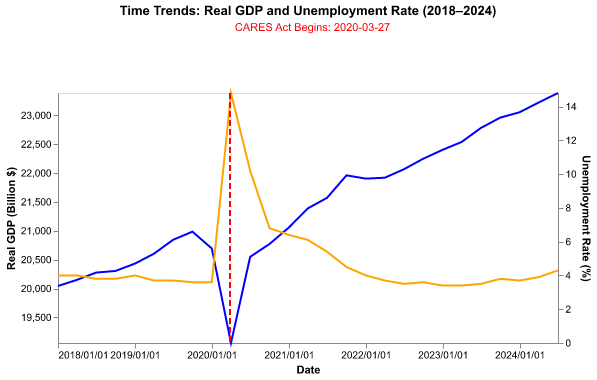
\includegraphics[width=6.21875in,height=3.95833in]{write_up_files/figure-pdf/cell-6-output-1.png}

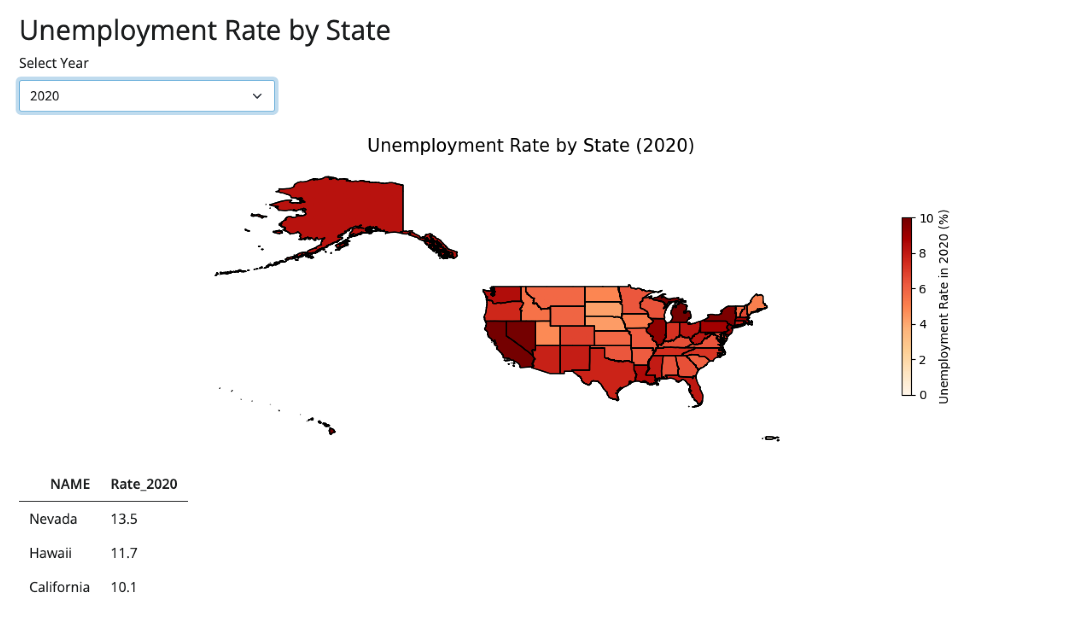
\includegraphics{write_up_files/figure-pdf/cell-15-output-1.pdf}

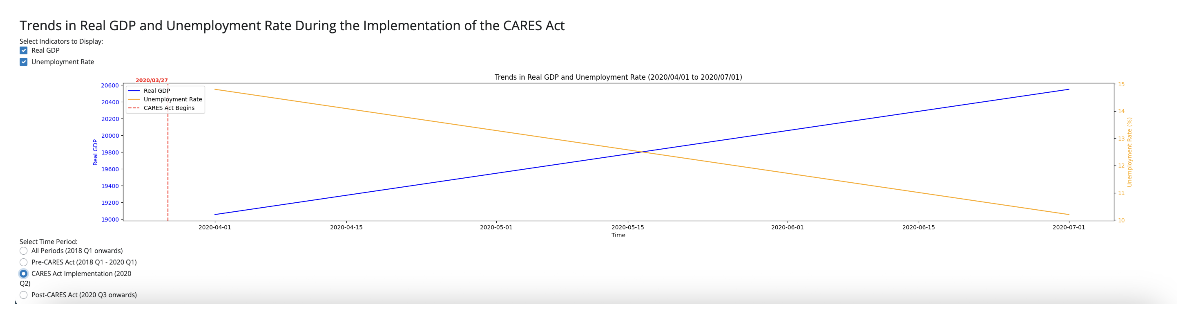
\includegraphics{write_up_files/figure-pdf/cell-16-output-1.pdf}

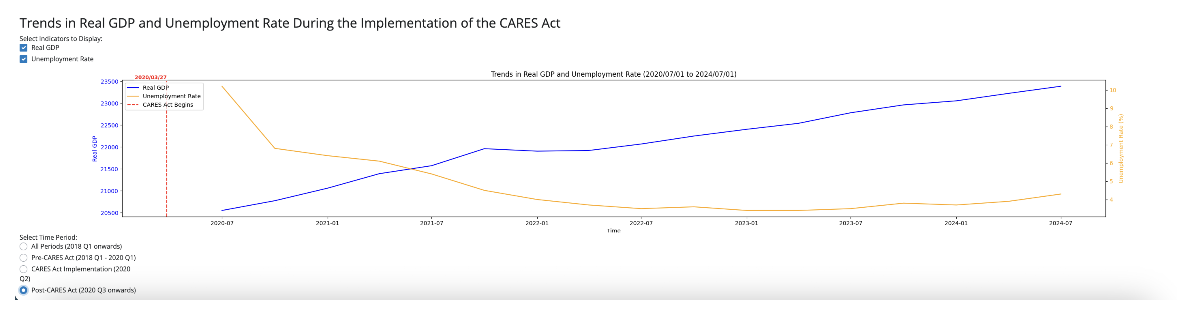
\includegraphics{write_up_files/figure-pdf/cell-16-output-2.pdf}




\end{document}
